% Choose one to switch between slides and handout
\documentclass[]{beamer}
%\documentclass[handout]{beamer}

% Video Meta Data
\title{Smart Contracts and Decentralized Finance}
\subtitle{Decentralized Exchange Protocols}
\author{Prof. Dr. Fabian Schär}
\institute{University of Basel}

% Config File
% Packages
\usepackage[utf8]{inputenc}
\usepackage{hyperref}
\usepackage{gitinfo2}
\usepackage{tikz}
 \usetikzlibrary{calc}
\usepackage{amsmath}
\usepackage{mathtools}
\usepackage{bibentry}
\usepackage{xcolor}
\usepackage{colortbl} % Add colour to LaTeX tables
\usepackage{caption}
\usepackage[export]{adjustbox}
\usepackage{pgfplots} \pgfplotsset{compat = 1.17}
\usepackage{makecell}
\usepackage{fancybox}
\usepackage{ragged2e}
\usepackage{fontawesome}
\usepackage{seqsplit}
\usepackage{tabularx}
\usepackage{tcolorbox}
\usepackage{booktabs} % use instead  \hline in tables

% Color Options
\definecolor{highlight}{rgb}{0.65,0.84,0.82}
\definecolor{focus}{rgb}{0.72, 0, 0}
\definecolor{lightred}{rgb}{0.8,0.5,0.5}
\definecolor{midgray}{RGB}{190,195,200}

 %UniBas Main Colors
\definecolor{mint}{RGB}{165,215,210}
\definecolor{anthracite}{RGB}{45,55,60}
\definecolor{red}{RGB}{210,5,55}

 %UniBas Color Palette (for graphics)
\definecolor{strongmint}{RGB}{30,165,165}
\definecolor{darkmint}{RGB}{0,110,110}
\definecolor{softanthracite}{RGB}{140,145,150}
\definecolor{brightanthracite}{RGB}{190,195,200}
\definecolor{softred}{RGB}{235,130,155}

%Custom Colors
\definecolor{lightergray}{RGB}{230, 230, 230}



% Beamer Template Options
\beamertemplatenavigationsymbolsempty
\setbeamertemplate{footline}[frame number]
\setbeamercolor{structure}{fg=black}
\setbeamercolor{footline}{fg=black}
\setbeamercolor{title}{fg=black}
\setbeamercolor{frametitle}{fg=black}
\setbeamercolor{item}{fg=black}
\setbeamercolor{}{fg=black}
\setbeamercolor{bibliography item}{fg=black}
\setbeamercolor*{bibliography entry title}{fg=black}
\setbeamercolor{alerted text}{fg=focus}
\setbeamertemplate{items}[square]
\setbeamertemplate{enumerate items}[default]
\captionsetup[figure]{labelfont={color=black},font={color=black}}
\captionsetup[table]{labelfont={color=black},font={color=black}}

\setbeamertemplate{bibliography item}{\insertbiblabel}

%tcolor boxes
\newtcolorbox{samplecode}[2][]{
  colback=mint, colframe=darkmint, coltitle=white,
  fontupper = \ttfamily\scriptsize, fonttitle= \bfseries\scriptsize,
  boxrule = 0mm, arc = 0mm,
  boxsep = 1.3mm, left = 0mm, right = 0mm, top = 0.5mm, bottom = 0mm, middle=0mm,
  #1,title=#2}
  
\newtcolorbox{keytakeaway}[2][]{
  colback=softred, colframe=red, coltitle=white,
  fontupper = \scriptsize, fonttitle= \bfseries\scriptsize,
  boxrule = 0mm, arc = 0mm,
  boxsep = 1.3mm, left = 0mm, right = 0mm, top = 0.5mm, bottom = 0mm, middle=0mm,
  #1,title=#2}

\newtcolorbox{exercise}[2][]{
  colback=brightanthracite, colframe=anthracite, coltitle=white,
  fontupper = \scriptsize, fonttitle= \bfseries\scriptsize,
  boxrule = 0mm, arc = 0mm,
  boxsep = 1.3mm, left = 0mm, right = 0mm, top = 0.5mm, bottom = 0mm, middle=0mm,
  #1,title=#2}



% Link Icon Command 
\newcommand{\link}{%
    \tikz[x=1.2ex, y=1.2ex, baseline=-0.05ex]{%
        \begin{scope}[x=1ex, y=1ex]
            \clip (-0.1,-0.1)
                --++ (-0, 1.2)
                --++ (0.6, 0)
                --++ (0, -0.6)
                --++ (0.6, 0)
                --++ (0, -1);
            \path[draw,
                line width = 0.5,
                rounded corners=0.5]
                (0,0) rectangle (1,1);
        \end{scope}
        \path[draw, line width = 0.5] (0.5, 0.5)
            -- (1, 1);
        \path[draw, line width = 0.5] (0.6, 1)
            -- (1, 1) -- (1, 0.6);
        }
    }

% Other commands
\newcommand\tab[1][0.5cm]{\hspace*{#1}} % for code boxes


% Read Git Data from Github Actions Workflow
% Defaults to gitinfo2 for local builds
\IfFileExists{gitInfo.txt}
	{\input{gitInfo.txt}}
	{
		\newcommand{\gitRelease}{(Local Release)}
		\newcommand{\gitSHA}{\gitHash}
		\newcommand{\gitDate}{\gitAuthorIsoDate}
	}

% Custom Titlepage
\defbeamertemplate*{title page}{customized}[1][]
{
  \vspace{-0cm}\hfill\includegraphics[width=2.5cm]{../config/logo_cif}
  \includegraphics[width=1.9cm]{../config/seal_wwz}
  \\ \vspace{2em}
  \usebeamerfont{title}\textbf{\inserttitle}\par
  \usebeamerfont{title}\usebeamercolor[fg]{title}\insertsubtitle\par  \vspace{1.5em}
  \small\usebeamerfont{author}\insertauthor\par
  \usebeamerfont{author}\insertinstitute\par \vspace{2em}
  \usebeamercolor[fg]{titlegraphic}\inserttitlegraphic
    \tiny \noindent \texttt{Release Ver.: \gitRelease}\\ 
    \texttt{Version Hash: \gitSHA}\\
    \texttt{Version Date: \gitDate}\\ \vspace{1em}
    
    
    \iffalse
  \link \href{https://github.com/cifunibas/Bitcoin-Blockchain-Cryptoassets/blob/main/slides/intro.pdf}
  {Get most recent version}\\
  \link \href{https://github.com/cifunibas/Bitcoin-Blockchain-Cryptoassets/blob/main/slides/intro.pdf}
  {Watch video lecture}\\ 
  
  \fi
  
  \vspace{1em}
  License: \texttt{Creative Commons Attribution-NonCommercial-ShareAlike 4.0 International}\\\vspace{2em}
  \includegraphics[width = 1.2cm]{../config/license}
}


% tikzlibraries
\usetikzlibrary{decorations.pathreplacing}
\usetikzlibrary{decorations.markings}
\usetikzlibrary{positioning}
\usetikzlibrary{calc}
\captionsetup{font=footnotesize}

%%%%%%%%%%%%%%%%%%%%%%%%%%%%%%%%%%%%%%%%%%%%%%
%%%%%%%%%%%%%%%%%%%%%%%%%%%%%%%%%%%%%%%%%%%%%%
\begin{document}

\thispagestyle{empty}
\begin{frame}[noframenumbering]
	\titlepage
\end{frame}


%%%
\begin{frame}{Exchanges}

	\begin{figure}[h!]
		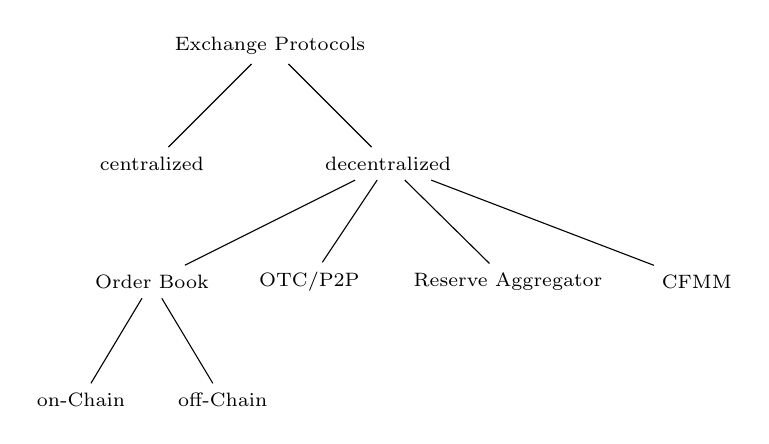
\begin{tikzpicture}
		[ sibling distance =10em ,
		every node/.style = {%shape=rectangle, rounded corners,
		%draw,
		font=\scriptsize,
		align = center,
		%top color=white, bottom color = highlight
		}]]
 		\tikzstyle{level 1}=[sibling distance=30mm]
 		\tikzstyle{level 2}=[sibling distance=20mm]
 		\tikzstyle{level 3}=[sibling distance=18mm]
  
  			\node {Exchange Protocols}
  			child { node {centralized}}
  			child { node {decentralized}
  				child { node {Order Book}
  					child { node {on-Chain}}
  					child { node {off-Chain}}}
  				child { node {OTC/P2P}}
  				child { node[right=-8mm] {Reserve Aggregator}}
  				child { node[right=1em] {CFMM}}
  			};
		\end{tikzpicture}
	\end{figure}
\uncover<2->{
	\begin{keytakeaway}{Problems}
		To be able to trade on a CEX, a users' funds must be deposited with the exchange. Thereby, access is forfeited and trust towards the exchange operator needed.  CEXs are also a single point of attack and face the constant threat of becoming the target of malicious third parties.
	\end{keytakeaway}
}	
\end{frame}
%%%


%%%
\begin{frame}{Decentralized Exchange Protocols}

\end{frame}
%%%


%%%
\begin{frame}{Constant Function Market Maker}

	\begin{figure}	
		\centering
		\begin{tikzpicture}
	
	% Pool
	\draw [thick] (-1,-1.5) -- (1,-1.5);
	\draw [thick](-1,-1.5) -- (-1, 0.6);
	\draw [thick](1,-1.5) -- (1, 0.6);
	\node [below=0.8cm] at (0,-0.8) {\scriptsize{Liquidity Pool}};
	
	% Balanced Pool
\uncover<2,3>{	
	\draw [fill=highlight] (-1,-1.5) rectangle (-0,0.25);
	\draw [fill=strongmint] (0,-1.5) rectangle (1,0.25);
}	

	% Unbalanced Pool
\uncover<4,5>{
	\draw [fill=highlight] (-1,-1.5) rectangle (-0,0);
	\draw [fill=strongmint] (0,-1.5) rectangle (1,0.5);
}	
\uncover<4>{
	\draw [dashed] (-1,0.25) -- (1,0.25);
}
	% Token labels
\uncover<2->{
\node at (-0.5,-0.7) {\scriptsize{CIF}};
\node at (0.5,-0.7) {\scriptsize{ETH}};
}

\uncover<4->{
 \node at (-4.5, 0.5) {\scriptsize{Pool Token}};
}
	
	%% LPs, Trader
	\uncover<1->{
		\node at (-4.5,-0.5) {\includegraphics[scale=0.03]{../assets/images/agents/agent_right}};
		\node at (-4,-0.8) {\includegraphics[scale=0.03]{../assets/images/agents/agent_right}};
		\node at (-5,-0.8) {\includegraphics[scale=0.03]{../assets/images/agents/agent_right}};
		\node [below=0.8cm] at (-4.5,-0.8) {\scriptsize{Liquidity Providers}};
		}
	\uncover<1->{
		\node at (4,-0.8) {\includegraphics[scale=0.05]{../assets/images/agents/agent_left}};
		\node [below=0.8cm]at (4,-0.8) {\scriptsize{Trader}};
		}
		
	%% Flow
	\uncover<2>{
		\draw[->] (-3.5, -0.8) -- (-1.5, -0.8) node [midway, below] {\includegraphics[scale=0.004]{../assets/images/eth}};
		\draw[->] (-3.5, -0.5) -- (-1.5, -0.5) node [midway, above]{\scriptsize{CIF}};
	}
	\uncover<3>{
	\draw[->] (-1.5, -0.8) -- (-3.5, -0.8) node [midway, above] {\scriptsize{Pool Token}};
	}
	\uncover<4>{
		\draw[->] (3.5, -0.8) -- (1.2, -0.8) node [midway, above] {\includegraphics[scale=0.004]{../assets/images/eth}};
		}

		
	\uncover<4>{
		\draw[->] (-0.5,0.12 ) arc (150:30:2.5cm) node [midway, above] {\scriptsize{CIF}};
	
		%\draw[dashed, <-] (-3.5,-2.5) arc (-130:-50:5.5cm) node [midway, above] {\scriptsize{Fees}};
	}
	
%	\uncover<5>{
%	\draw (0,1) node {\scriptsize{\textcolor{focus}{Arbitrage Opportunity}}};
%	\draw[-] (-0.25,0.8) -- (-0.25,0.25);
%	\draw[->] (-0.25,0.25) -- (0,0.25);
%	
%	}
		
	\end{tikzpicture}
	\end{figure}

\uncover<5->{
	\begin{itemize}
		\item The price is determined endogenously via a formula. There are different types of formulas.
		\item Traders pay a fee, this fee is subtracted in the formula. Fees are needed to incentivize Liquidity Providers.
		\item When the pool price differs from the market price (e.g on a centralized exchange), there is an arbitrage opportunity. This keeps the price up to date (in line with Market Price).
	\end{itemize}
}

\end{frame}
%%%


%%%
\begin{frame}{Constant Product Formula}
	\only<1-4>{
		\begin{align*}
			k &= x \cdot y
		\end{align*}
	}
	\only<1>{
		\begin{itemize}
			\item k: constant
			\item x: number of x-tokens in the pool
			\item y: number of y-tokens in the pool
		\end{itemize}
		\vspace{0.5cm}
	}

	\only<2-4>{\textbf{Properties:}}
	\begin{itemize}
		\item<3-4> Convexity of the indifference set
		\item<4> Dynamic endogenous pricing model
	\end{itemize}
	
	\only<5>{
		\begin{figure}[h!]
			\begin{center}
				\begin{tikzpicture}[]
    
    \draw[samples = 200, color=blue, scale=1, xshift = 0cm, yshift = 0cm, domain=0.9:4.55, smooth, variable=\x] plot ({\x}, {4/\x}) node[right,color=blue] {$k$} ;       
    
  	\draw[->] (0,0)--(5,0) node[below,midway]{} node[right] {$X$-tokens in liquidity pool} ;
    \draw[->] (0,0)--(0,5) node[above,midway,rotate=90]{} node[above] {$Y$-tokens in liquidity pool};  
  
    \draw[dotted, thick] (2,2)--(0,2) node[left]{\scriptsize $y$};

    \draw[dotted, thick] (2,2)--(2,0) node[below, yshift = -0.08cm]{\scriptsize $x$};
  
	\draw[fill=black] (2,2) circle(2pt);

\end{tikzpicture}
			\end{center}
		\end{figure}
	}
\end{frame}
%%%

%%%
\begin{frame}{AMM Functions}
	\begin{itemize}
		\item<1-> swap():
		\item<2-> mint():
		\item<3-> burn(): 
	\end{itemize}
\end{frame}
%%%

%%%
\begin{frame}{Swap (without fees)}
	\only<1>{
		\begin{figure}[h!]
			\begin{center}
				\begin{tikzpicture}[]
    
    \draw[samples = 200, color=blue, scale=1, xshift = 0cm, yshift = 0cm, domain=0.9:4.55, smooth, variable=\x] plot ({\x}, {4/\x}) node[right,color=blue] {$k$} ;       
    
  	\draw[->] (0,0)--(5,0) node[below,midway]{} node[right] {$x$-tokens} ;
    \draw[->] (0,0)--(0,5) node[above,midway,rotate=90]{} node[above] {$y$-tokens};  
  
  	% Before Swap
    \draw[dotted, thick] (2,2)--(0,2) node[left]{\scriptsize $y$};
    \draw[dotted, thick] (2,2)--(2,0) node[below, yshift = -0.08cm]{\scriptsize $x$};
	\draw[fill=black] (2,2) circle(2pt);
	
	% After Swap
    \draw[dotted, thick] (3,1.333)--(0,1.333) node[left]{\scriptsize $y-\Delta(y)$};	
    \draw[dotted, thick] (3,1.333)--(3,0) node[below]{\scriptsize $x+\Delta(x)$};
	\draw[fill=black] (3,1.333) circle(2pt);

\end{tikzpicture}
			\end{center}
		\end{figure}
	}

	\only<2>{
		\begin{align*}
			k &= (x + \Delta x) \cdot (y - \Delta y) \\
			\Delta y &= y - \biggl( \frac{k}{x + \Delta x} \biggr)
		\end{align*}
		
		\begin{itemize}
			\item TODO: Explain slippage and relation to trade size / pool size
		\end{itemize}
	}

\end{frame}
%%%


%%%
\begin{frame}{Swap (with fees)}
	\begin{tikzpicture}[]
    
 	\draw[->] (0,0)--(5,0) node[below,midway]{} node[right] {$x$-tokens} ;%{\small{$x$-tokens in liquidity pool}};
	\draw[->] (0,0)--(0,5) node[above,midway,rotate=90]{} node[above] {$y$-tokens};%{\small{$y$-tokens in liquidity pool}};

	% k before swap
 	\draw[samples = 200, color=blue, scale=1, xshift = 0cm, yshift = 0cm, domain=0.9:4.55, smooth, variable=\x] plot ({\x}, {4/\x}) node[right,color=blue] {$k$} ;    

	% k after swap
 	\draw[samples = 200, color=blue, scale=1, xshift = 0cm, yshift = 0cm, domain=1.345:4.55, smooth, variable=\x] plot ({\x}, {6/\x}) node[right,color=blue] {$k'$} ;    
	 
	% reserves before swap
	\draw[fill=black] (1.75,2.3) circle(2pt);
	\draw[dotted,thick] (1.75,2.3) -- (1.75,0) node[below]{\scriptsize{${x}$}};
	\draw[dotted,thick] (1.75,2.3) -- (0,2.3) node[left]{\scriptsize{$y$}};
	
	% reserves after swap (incl. fees)
	\draw[fill=black] (3.5,1.715) circle(2pt);
	\draw[dotted,thick] (3.5,1.715) -- (3.5,0) node[below]{\scriptsize{${x+\Delta(x)}$}};
	\draw[dotted,thick] (3.5,1.715) -- (0,1.715) node[left]{\scriptsize{${y-\Delta(y_\rho)}$}};
	
	% reserves after swap (excl. fees)
	\draw[dotted,thick] (3.5,1.13) -- (0,1.13) node[left]{\scriptsize{${y-\Delta(y_\rho)-\tau}$}};
 
\end{tikzpicture}
\end{frame}
%%%


%%%
\begin{frame}{Liquidity Provision}

\end{frame}
%%%


%%%
\begin{frame}{Divergence Loss}

\end{frame}
%%%


%%%
\begin{frame}{Swap Example}

\textbf{Swap one x-token with a fee of 0.3 \%} \\ \vspace{1.5em}

	\begin{minipage}{0.5\textwidth}
		\begin{figure}[h!]
			\begin{center}
 				\begin{tikzpicture}[]
    
 	\draw[->] (0,0)--(5,0) node[below,midway]{} node[below, midway, yshift = -0.5cm] {\small{$X$-tokens in LP}};	
 	\draw[->] (0,0)--(0,5) node[above,midway,rotate=90]{} node[above] {\small{$Y$-tokens in LP}};

	% Initial reserves
 	\draw[samples = 200, color=blue, scale=1, xshift = 0cm, yshift = 0cm, domain=0.9:4.55, smooth, variable=\x] plot ({\x}, {4/\x}) node[right, below] {\scriptsize{$k$}} ;    
    \draw[dotted, thick] (2,2)--(0,2) node[left]{\scriptsize 10};
    \draw[dotted, thick] (2,2)--(2,0) node[below]{\scriptsize 10};
	\draw[red, fill=red] (2,2) circle(1.2pt);

	% Delta x
	\only<2>{
		\draw[->, red] (2.05, 0.1) -- (2.95, 0.1) node [midway, above] {\scriptsize{5}};	
	}
	\only<2 | handout:0>{
		\draw[dotted,thick] (3,1.3) -- (3,0) node[below]{\scriptsize{15}};	
	}
	\uncover<3-5>{
		\draw[dotted,thick] (3,1.3) -- (3,0) node[below]{};
	}
	
	% Delta x minus fees
	\uncover<3-4>{
		\draw[dotted, red, thick] (2.8,1.43) -- (2.8,0) node[below]{\scriptsize{14}};

	}
	\uncover<3-4>{
		\draw[->, red] (2.95, 0.625) -- (2.85, 0.625) node {};	
	}
	
	% y'
	\uncover<4 | handout:0>{	
		\draw[dotted,thick] (2.8,1.43) -- (0,1.43) node[left]{\scriptsize{$7.1429$}};
	}
	
	% k'
	\uncover<5->{
		\draw[samples = 200, color=blue, scale=1, xshift = 0cm, yshift = 0cm, domain=0.97:4.55, smooth, variable=\x] plot ({\x}, {4.3/\x}) node[right, above] {\scriptsize{$k'_\rho$}};

		\draw[dotted,thick] (3,1.43) -- (0,1.43) node[left]{\scriptsize{$7.1429$}};
		\draw[dotted, red, thick] (2.8,1.43) -- (2.8,0) node[below]{};
		\draw[red, fill=red] (3,1.43) circle(1.2pt);
		\draw[->, blue] (4.63, 0.85) -- (4.63, 1.0) node {};		
	}	
	\uncover<5- | handout:0>{
		\draw[dotted,thick] (3,1.3) -- (3,0) node[below]{\scriptsize{15}};	
	}
\end{tikzpicture}
			\end{center}
		\end{figure}
	\end{minipage}
\vspace{1em}
	\begin{minipage}{0.4\textwidth}
		\vspace{-4em}
		\begin{scriptsize}
			\begin{align*}
			\only<1>{
				\Delta (y) &= \dfrac{k}{x+ (1-\tau) \Delta (x)} - y \\
			}
			\only<2>{
			 	\Delta (y) &= \dfrac{100}{10+ (1-0.003) \cdot 10} - 10 \\
		 		&= -0.9066 \\
		 	}
		 	\only<3>{
		 		y' &= 10 - 0.9066 = 9.0934 \\
		 		k' &= 11 \cdot 9.0934 = 100.0274 \\
			}
			\only<4>{
				PR &= \dfrac{y}{x} = 10/10 = 1 \\
				P_{eff} &= \dfrac{\Delta (y)}{\Delta (x)} = \dfrac{0.9066}{1} = 0.9066\\
				PR' &= \dfrac{y'}{x'} = \dfrac{9.0934}{11} =  0.8267 \\
			}
			\only<5>{
				S &= \dfrac{P_{eff}}{PR} - 1 = \dfrac{0.9066}{1} - 1 = -0.0934 \\
			}
			\end{align*}
		\end{scriptsize}
	\end{minipage}

\end{frame}
%%%


%%%
\begin{frame}{Swap Example 2}
	\textbf{Swap one x-token with a fee of 0.3 \%} \\

	\begin{minipage}{0.5\textwidth}
		\begin{figure}[h!]
			\begin{center}
				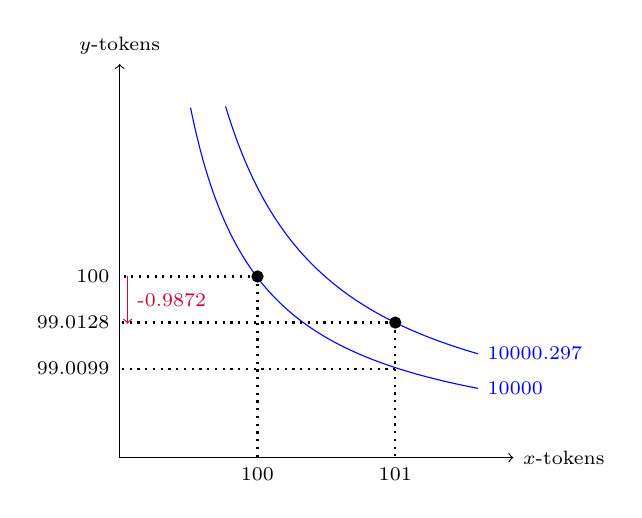
\begin{tikzpicture}[]
    
 	\draw[->] (0,0)--(5,0) node[below,midway]{} node[right] {\scriptsize{$x$-tokens}} ;%{\small{$x$-tokens in liquidity pool}};
	\draw[->] (0,0)--(0,5) node[above,midway,rotate=90]{} node[above] {\scriptsize{$y$-tokens}};%{\small{$y$-tokens in liquidity pool}};

	% k before swap
 	\draw[samples = 200, color=blue, scale=1, xshift = 0cm, yshift = 0cm, domain=0.9:4.55, smooth, variable=\x] plot ({\x}, {4/\x}) node[right,color=blue] {\scriptsize{10000}} ;    

	% k after swap
 	\draw[samples = 200, color=blue, scale=1, xshift = 0cm, yshift = 0cm, domain=1.345:4.55, smooth, variable=\x] plot ({\x}, {6/\x}) node[right,color=blue] {\scriptsize{10000.297}} ;    
	 
	% reserves before swap
	\draw[fill=black] (1.75,2.3) circle(2pt);
	\draw[dotted,thick] (1.75,2.3) -- (1.75,0) node[below]{\scriptsize{100}};
	\draw[dotted,thick] (1.75,2.3) -- (0,2.3) node[left]{\scriptsize{100}};
	
	% reserves after swap (incl. fees)
	\draw[fill=black] (3.5,1.715) circle(2pt);
	\draw[dotted,thick] (3.5,1.715) -- (3.5,0) node[below]{\scriptsize{101}};
	\draw[dotted,thick] (3.5,1.715) -- (0,1.715) node[left]{\scriptsize{99.0128}};
	\draw[->, red] (0.1, 2.3) -- (0.1, 1.7) node [midway, right] {\scriptsize{-0.9872}};
	
	% reserves after swap (excl. fees)
	\draw[dotted,thick] (3.5,1.13) -- (0,1.13) node[left]{\scriptsize{99.0099}};
 
\end{tikzpicture}
			\end{center}
		\end{figure}
	\end{minipage}
\vspace{1em}
	\begin{minipage}{0.4\textwidth}
		\vspace{-4em}
		\begin{scriptsize}
			\begin{align*}
			\only<1>{
				PR &= \dfrac{y}{x} = 100/100 = 1 \\
				P_{eff} &= \dfrac{\Delta (y)}{\Delta (x)} = \dfrac{0.9872}{1} = 0.9872\\
				PR' &= \dfrac{y'}{x'} = \dfrac{99.0128}{101} =  0.9803 \\
			}
			\only<2>{
				S &= \dfrac{P_{eff}}{PR} - 1 = \dfrac{0.9872}{1} - 1 = -0.0128 \\
			}
			\end{align*}
		\end{scriptsize}
	\end{minipage}
	
	\uncover<2>{When the trade size is smaller compared to the pool liquidity, slippage is also reduced. In our example from $\approx$ 10\% to $\approx$ 1.3\%.
	}
		
\end{frame}
%%%


%%%
\begin{frame}{Divergence Loss Example}
	Liquidity Provision, Divergence Loss Example
\end{frame}
%%%


%%%
\begin{frame}{Different Functions (Curve)}

\end{frame}
%%%


%%%
\begin{frame}{Concentrated Liquidity}

\end{frame}
%%%


%%%
\begin{frame}{n $>$ 2 Pool Assets}

\end{frame}
%%%


%%%
\begin{frame}{Concept of Aggregators}

\end{frame}
%%%


%%%
\begin{frame}{Frontrunning}

\end{frame}
%%%


%%%
\begin{frame}{Add. Liquidity Mining \& Vampire Attack}

\end{frame}
%%%


%%%
\begin{frame}{Initial DEX offerings}

\end{frame}
%%%


%%%
\begin{frame}{Exercise}
	\begin{exercise}{Exercise 1}
	For this exercise we use the ERC20 Token created in one of the previous videos (select Ropsten). Go two UniSwap Frontend Link to complete the following tasks:
	
		\begin{enumerate}
			\item Swap ETH to CIF
			\item Provide liquidity to ETH/CIF Pool
			\item Make another Swap
			\item Remove your liquidity position and analyze what happened
		\end{enumerate}
	\end{exercise}
\end{frame}
%%%



%%%
\begin{frame}%[allowframebreaks]
\frametitle{References and Recommended Reading}
	\bibliographystyle{amsplain}
	\bibliography{../assets/bib/refs}
\end{frame}
%%%





\end{document}